%  UWSTHESIS sample file
%
%% Some things about references, referencing is essentially APA style, and this is hard coded, it can be changed in
%% the .cls file, 
%% a note on references, currently the code here uses two files (whose names are hard coded)
%% references.bib -- contains the references that are cited in the text => References Section
%% bibliography.bib -- contains the references that aren't cited but would be nice => Bibliography sec.
%% to get it all to work ,TeXShop (for mac, YMMV) can't handle it (the mix of classes confuses it), you need to run BiBTeX
%% by hand. Open a terminal and change to the directory that your work is in and type:
%%
%%  for f in *.aux; do bibtex ${f%.*}; done
%%
%%  this little loop will bibtex everything for you, and then run latex/pdflatex a few more times to fix
%%  A python script split_refs.py is provided, and included below, read the source to understand how to use it
%% it parses the .aux file to extract the references, and produces a file bibliography.bib file that contains the entries
%% not cited from references.bib, its rough but it works.
%
%
%% This class uses hyperref, so that tables of contents, lists of XXX, citations and cross references all become hyperlinks in
%% the pdf produced. The boxes produced are not printed, but are clickable in the electronic version.
%
%
%% options below controls degree submitted for
%% 	    -  bithns             -- Bachelor of Information Technology (Honours)
%% 	    -  comphns       -- Bachelor of Computing (Honours)
%% 	    -  compscihns  -- Bachelor of Computer Science (Honours)
%% 	    -  scimathns     --  Bachelor of Science Mathematics (Honours)
%% 	    -  msc                -- Master of Science (Honours)
%%      -  mphil             -- Master of Philosophy
%%      -  mres              -- Master of Research
%% 	    -  phd (default) -- Doctor of Philosophy

%% options coc or thesis (default) controls type of monograph
%% options nocopy or copy (default) don't put/put a copyright notice on the title page
%% options nologo or logo (default) don't put/put a logo notice on the title page
%% options nosoo or soo (default) don't put/put a Statement Of Originality (you probably should accept the default here)
%% options nolot or lot (default) controls the list of tables, use nolot if you dont have any, as lot will still produce an empty list
%% options nolof or lof (default) controls the list of figures, use nolof if you dont have any, as lof will still produce an empty list
%% options nobib or bib (default) controlls the activation of the bibliography, a list of supplementary materials not directly referenced.

\documentclass[twoside,phd,thesis,copy,soo,lof,lot]{uwsthesis}
\title{A Multifrequency Study of the Magellanic Clouds}
\author{Evan Johnston Crawford}
%date of submission, day, month, year as numbers
\subdate{15}{2}{2019}

%% Most of the text below comes from  OUTLINE SCIENCE, that I got from Project Gutenburg. Other bits are examples,
%% look at the typset version first to see the examples then the code!


%% dedication -- optional -- text to appear in the Dedication section
%% comment it out like the acknowledgements below to disable
\dedication{There is abundant evidence of a widened and deepened interest in modernscience. How could it be otherwise when we think of the magnitude and the eventfulness of recent advances?}


%% acknowledgements -- optional -- text to appear in the Acknowledgements section
%\acknowledgements{There is abundant evidence of a widened and deepened interest in modern science. How could it be otherwise when we think of the magnitude and the eventfulness of recent advances?}


%% supervisors, a comma separated list of supervisors, will appear on cover if defined
\supervisors{Prof. A. Einstein (Western Sydney University), Dr Doom (Latveria University) , Dr Jane Goodall, and more}

%% abstract -- mandatory -- text to appear in the abstract
\abstract{There is abundant evidence of a widened and deepened interest in modern
science. How could it be otherwise when we think of the magnitude and
the eventfulness of recent advances?

But the interest of the general public would be even greater than it is
if the makers of new knowledge were more willing to expound their
discoveries in ways that could be "understanded of the people." No one
objects very much to technicalities in a game or on board a yacht, and
they are clearly necessary for terse and precise scientific description.
It is certain, however, that they can be reduced to a minimum without
sacrificing accuracy, when the object in view is to explain "the gist of
the matter." So this OUTLINE OF SCIENCE is meant for the general reader,
who lacks both time and opportunity for special study, and yet would
take an intelligent interest in the progress of science which is making
the world always new.
}

%% acronyms are mandatory at the moment (i'll make them optional if requested)
% The acronyms need to be sorted by hand, as the code isn't smart enough to do it for you
% but the sample list is unsorted, (Hey i'm lazy)
% MMMM controlls the with of abbrev col (put the same number of M's as the longest abbrev), if an abbrev is too long
% then the list will still work it just wont be neat. 
\acronymlist{MMMM}{
\acro{MC}{Magellanic Cloud}
\acro{LMC}{Large Magellanic Cloud}
\acro{SMC}{Small Magellanic Cloud}
\acro{ATNF}{Australia Telescope National Facility}
\acro{ATCA}{Australia Telescope Compact Array}
\acro{RA}{Right Ascension}
\acro{DEC}{Declination}
\acro{SI}[$\alpha$]{Spectral index}
}



%document begins here
\begin{document}
\frontstuff   %% this put the front stuff in the form required by the UWS style guide
%% create parts and chapters here
%\part{FIRST PART}
\chapter{Preface}
A first chapter.
\chapter{Introduction}
\section{The First Section}
This is the first section.

\subsection{The First Subsection}
This is the first subsection.
\section{Acronym Test}
These are acronyms, \ac{MC}, introduced for the first time, and the second: \ac{MC}. Some others:
\ac{LMC}, \ac{SMC}, \ac{ATNF}, \ac{ATCA}, \ac{RA} and \ac{DEC}. 

The second use of the others:
\ac{LMC}, \ac{SMC}, \ac{ATNF}, \ac{ATCA}, \ac{RA} and \ac{DEC}. 

Note that the abbreviation for this one is different to its display, look above for how to do this. First time: \ac{SI}, and second \ac{SI}.

\section{A figure}
An image figure appears next but \LaTeX\ will put it where it wants.

\begin{figure}[h]
%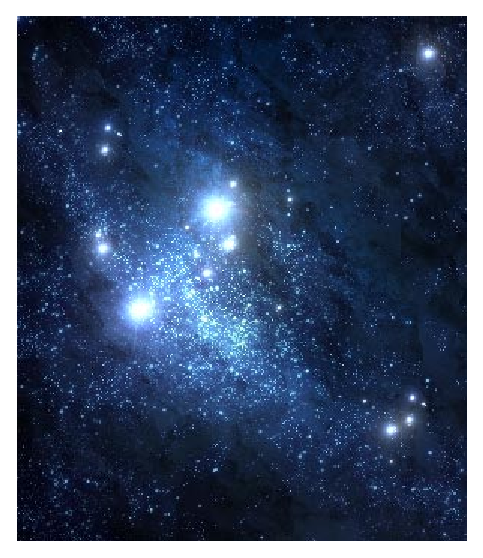
\includegraphics[width=\textwidth]{12}
\centering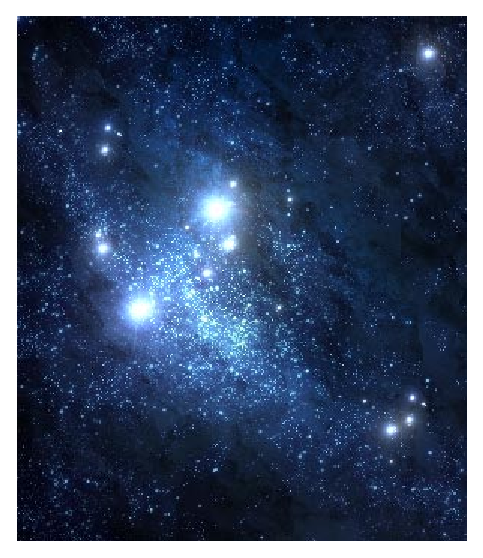
\includegraphics{12}
%% A note on graphics, with latex graphics should be in encapsulated postscript (eps) format
%% if you use pdflatex, then graphics can be pdf, jpg or png (the eps can be converted to pdf)
%% The example graphic is provided in both formats.
% A note on style, typically journals want image/graph captions below the image and tables above,
% the position of the \caption{} command determines this, see the table below for the opposite.
\caption{A figure}
\end{figure}


\emph{The rest of this chapter is junk text to pad it out.}

The story of the triumphs of modern science is one of which Man may well
be proud. Science reads the secret of the distant star and anatomises
the atom; foretells the date of the comet's return and predicts the
kinds of chickens that will hatch from a dozen eggs; discovers the laws
of the wind that bloweth where it listeth and reduces to order the
disorder of disease. Science is always setting forth on Columbus
voyages, discovering new worlds and conquering them by understanding.
For Knowledge means Foresight and Foresight means Power.

The idea of Evolution has influenced all the sciences, forcing us to
far since Darwin's day. The solar system, the earth, the mountain
ranges, and the great deeps, the rocks and crystals, the plants and
animals, man himself and his social institutions--all must be seen as
the outcome of a long process of Becoming. There are some eighty-odd
chemical elements on the earth to-day, and it is now much more than a
suggestion that these are the outcome of an inorganic evolution, element
giving rise to element, going back and back to some primeval stuff, from
which they were all originally derived, infinitely long ago. No idea has
been so powerful a tool in the fashioning of New Knowledge as this
simple but profound idea of Evolution, that the present is the child of
the past and the parent of the future. And with the picture of a
continuity of evolution from nebula to social systems comes a promise of
an increasing control--a promise that Man will become not only a more
accurate student, but a more complete master of his world.
\section{Two}
It is characteristic of modern science that the whole world is seen to
be more vital than before. Everywhere there has been a passage from the
static to the dynamic. Thus the new revelations of the constitution of
matter, which we owe to the discoveries of men like Professor Sir J. J.
Thomson, Professor Sir Ernest Rutherford, and Professor Frederick Soddy,
have shown the very dust to have a complexity and an activity heretofore
unimagined. Such phrases as "dead" matter and "inert" matter have gone
by the board.

The new theory of the atom amounts almost to a new conception of the
universe. It bids fair to reveal to us many of nature's hidden secrets.
The atom is no longer the indivisible particle of matter it was once
understood to be. We know now that there is an atom within the
atom--that what we thought was elementary can be dissociated and broken
up. The present-day theories of the atom and the constitution of matter
are the outcome of the comparatively recent discovery of such things as
radium, the X-rays, and the wonderful revelations of such instruments as
the spectroscope and other highly perfected scientific instruments.

The advent of the electron theory has thrown a flood of light on what
before was hidden or only dimly guessed at. It has given us a new
conception of the framework of the universe. We are beginning to know
and realise of what matter is made and what electric phenomena mean. We
can glimpse the vast stores of energy locked up in matter. The new
knowledge has much to tell us about the origin and phenomena, not only
of our own planet, but other planets, of the stars, and the sun. New
light is thrown on the source of the sun's heat; we can make more than
guesses as to its probable age. The great question to-day is: is there
have been evolved?

But the discovery of electrons is only one of the revolutionary changes
which give modern science an entrancing interest.
\chapter{Other Things}
\section{A table}
A table is defined here, but \LaTeX\ will put it where it wants (just like the figure).

\begin{table}
% A note on style, typically journals want image/graph captions below the image and tables above,
% the position of the \caption{} command determines this, see the figure above for the opposite.
\begin{center}
\caption[A table for the list of tables]{A Table for the caption}
%% Caption accepts 2 arguments, the optional one for the List of and the mandatory one for the caption.
%% if you leave out the optional one, then the mandatory one is used in both places (see the figure above)
\begin{tabular}{cc}
\hline
Col 1 & Col 2 \\
\hline
blah & blah \\
blah & blah \\
blah & blah \\
blah & blah \\
blah & blah \\
blah & blah \\
\hline
\end{tabular}
\end{center}
\end{table}


\section{Referencing Fun}
This is a first reference \citep{2008A&A...485...63F} is in parenthesis. The next is in text, viz \citet{2008SerAJ.177...61C} say something really interesting. You can also add bits before and after \citep[before][after]{2008arXiv0806.3605D} but you should use it for things like \citep[][section 2]{2008arXiv0806.3605D} or \citep[][page 7]{2008SerAJ.177...61C}. See the \textsf{natbib} package documentation for more information.


\section{The \texttt{split\_refs.py} script}



This uses the \textsf{listings} package to format the code, see the CTAN documentation for details on how to control how the code looks.

%\singlespacing

\begin{lstlisting}[language=python,breaklines=false]
#!/usr/bin/env python

import sys


if len(sys.argv) != 2:
	print "Usage: split_ref.py filename"
	sys.exit()

refs={}
f=open("references.bib")
n=f.read()
f.close()
o=n.split('@')
for p in o:
	if p and not p.startswith('%'):
		key=p.split('{')[1].split(',')[0]
		refs[key]=p


#print refs


f2=open("%s.aux"%sys.argv[1].split('.')[0])
cited=f2.read().split('\n')
f2.close()

for l in cited:
	if l.startswith("\citation{"):
		key=l.split('{')[1].split('}')[0]
#		print key
		if key.find(',')>=0:
			print 'many'
			for nkey in key.split(','):
				if nkey in refs:
					del refs[nkey]
		else:
			if key in refs:
				del refs[key]
import os
os.system("cp bibliography.bib bibliography-%i.bib"%os.getpid())
f3=open("bibliography.bib","w")
for k in refs:
	f3.write( "@%s" % refs[k])
f3.close()
\end{lstlisting}


\section{Padding Text}
\emph{The rest of this chapter is junk text to pad out the pages.}

The story of the triumphs of modern science naturally opens with
Astronomy. The picture of the Universe which the astronomer offers to us
is imperfect; the lines he traces are often faint and uncertain. There
are many problems which have been solved, there are just as many about
which there is doubt, and notwithstanding our great increase in
knowledge, there remain just as many which are entirely unsolved.

    The problem of the structure and duration of the universe [said the
    great astronomer Simon Newcomb] is the most far-reaching with which
    the mind has to deal. Its solution may be regarded as the ultimate
    object of stellar astronomy, the possibility of reaching which has
    occupied the minds of thinkers since the beginning of civilisation.
    Before our time the problem could be considered only from the
    imaginative or the speculative point of view. Although we can to-day
    attack it to a limited extent by scientific methods, it must be
    admitted that we have scarcely taken more than the first step toward
    the actual solution.... What is the duration of the universe in
    time? Is it fitted to last for ever in its present form, or does it
    contain within itself the seeds of dissolution? Must it, in the
    course of time, in we know not how many millions of ages, be
    transformed into something very different from what it now is? This
    question is intimately associated with the question whether the
    stars form a system. If they do, we may suppose that system to be
    permanent in its general features; if not, we must look further for
    our conclusions.


\section{The Heavenly Bodies}
The heavenly bodies fall into two very distinct classes so far as their
relation to our Earth is concerned; the one class, a very small one,
comprises a sort of colony of which the Earth is a member. These bodies
the Earth, and they all circle round the sun. Their names, in the order
of their distance from the sun, are Mercury, Venus, Earth, Mars,
Jupiter, Saturn, Uranus, Neptune, and of these Mercury, the nearest to
the sun, is rarely seen by the naked eye. Uranus is practically
invisible, and Neptune quite so. These eight planets, together with the
sun, constitute, as we have said, a sort of little colony; this colony
is called the Solar System.



solar system. Every one of those glittering points we see on a starlit
night is at an immensely greater distance from us than is any member of
the Solar System. Yet the members of this little colony of ours, judged
by terrestrial standards, are at enormous distances from one another. If
a shell were shot in a straight line from one side of Neptune's orbit to
the other it would take five hundred years to complete its journey. Yet
this distance, the greatest in the Solar System as now known (excepting
the far swing of some of the comets), is insignificant compared to the
distances of the stars. One of the nearest stars to the earth that we
know of is Alpha Centauri, estimated to be some twenty-five million
millions of miles away. Sirius, the brightest star in the firmament, is
double this distance from the earth.

We must imagine the colony of planets to which we belong as a compact
little family swimming in an immense void. At distances which would take
our shell, not hundreds, but millions of years to traverse, we reach
the stars--or rather, a star, for the distances between stars are as
great as the distance between the nearest of them and our Sun. The
Earth, the planet on which we live, is a mighty globe bounded by a crust
of rock many miles in thickness; the great volumes of water which we
call our oceans lie in the deeper hollows of the crust. Above the
surface an ocean of invisible gas, the atmosphere, rises to a height of
about three hundred miles, getting thinner and thinner as it ascends.


\bibandref %% this does the references and bibliography
%\backmatter
\appendix
%% put Glossary, Appendicies and Index here, for appendicies start a new chapter, for the others
%% your on your own but I'll try to help if needed.
\appendix

\chapter{This is an example appendix}
This is the appendix.
\chapter{Another Example}
This is a second example.
\end{document}
